\documentclass[colorinlistoftodos]{article}

% if you need to pass options to natbib, use, e.g.:
% \PassOptionsToPackage{numbers, compress}{natbib}
% before loading nips_2018

\usepackage[final]{nips_2018}

\usepackage[utf8]{inputenc} % allow utf-8 input
\usepackage[T1]{fontenc}    % use 8-bit T1 fonts
\usepackage{hyperref}       % hyperlinks
\usepackage{url}            % simple URL typesetting
\usepackage{booktabs}       % professional-quality tables
\usepackage{amsfonts}       % blackboard math symbols
\usepackage{nicefrac}       % compact symbols for 1/2, etc.
\usepackage{microtype}      % microtypography


%-----------------------------------------------------------------
\usepackage{pdfpages}
\usepackage{float}
\usepackage{tikz}
\usetikzlibrary{positioning}
\usetikzlibrary{calc}

\usepackage{amssymb,amsmath}
\usepackage{mathtools}

\usepackage{color}
\usepackage[font=small,labelfont=bf]{caption}
%----------------
\usepackage{algorithm,algorithmicx,algpseudocode}
\algnewcommand\algorithmicinput{\textbf{Input:}}
\algnewcommand\INPUT{\item[\algorithmicinput]}
\algnewcommand\algorithmicoutput{\textbf{Output:}}
\algnewcommand\OUTPUT{\item[\algorithmicoutput]}
\algnewcommand\algorithmicidea{\textbf{Idea:}}
\algnewcommand\IDEA{\item[\algorithmicidea]}
\algnewcommand\algorithmicinit{\textbf{Initialize:}}
\algnewcommand\INIT{\item[\algorithmicinit]}
%----------------

\usepackage{amsthm}

\providecommand{\tightlist}{%
  \setlength{\itemsep}{0pt}\setlength{\parskip}{0pt}}

\usepackage{fancyvrb}

% pandoc tmp.markdown -t latex -o tmp.tex

\theoremstyle{definition}
\newtheorem{definition}{Definition}[section]
\def\R{\mathbb{R}}

\usepackage{todonotes}
\newcommand{\rob}[1]{\todo[color=red!40]{Rob: #1}}
%-----------------------------------------------------------------
\title{Biologically Plausible Deep Learning: \\
		A Critical Review}

\author{
  Robert T. Lange \thanks{This progress report was submitted as part of the final project of the "Models of Neural Systems" (Winter Term 2018/2019) computer practical course taught and organized by Prof. Richard Kempter (Bernstein Center for Computational Neuroscience, Berlin).} \\
  Einstein Center for Neurosciences Berlin\\
  \url{robert.lange17@imperial.ac.uk} \\
  \url{www.rob-lange.com} \\
}

\begin{document}


\maketitle

%--------------------------------------------------------------------


%--------------------------------------------------------------------
\section{Introduction}

Backpropagation \citep{rumelhart1986} provides a biologically implausible solution to the synaptic credit assignment problem in Deep Learning (see e.g. \citet{lecun2015, schmidhuber2015}). While computational graphs and the chain rule successfully provide approximate gradients in deep layered structures, the mere empirical success does not imply that the brain is capable of implementing such a procedure.\rob{Restructure Introduction!}
In this report we review different proposed solutions to such problems that render backpropagation biologically implausible. More specifically, we focus on an approach which implements local plasticity rules in a neural network architecture with dendritic compartments \citep{guerguiev2017}.
Previously it has been argued that such an architecture overcomes multiple points of critique while accomplishing similar strong results. Our robustness checks reveal that such a claim is not justified.
Deep Learning (DL) has rightfully been the poster child of Machine Learning success in the 21st century. It has dominated competitions and research across all domains (computer vision, natural language processing, robotics as well as computational neuroscience).

Kriegeskorte/DiCarlo/RSA - DNNs outperform alternative frameworks in accurately reproducing activity patterns in cortex - What does this mean? Is DL just extremely flexible/expressive?

The report is structured as follows: First, we set the stage by introducing notation as well as fundamental problems with backpropagation. 
We briefly review the literature trying to solve such.
Afterwards, we introduce the local compartmental learning paradigm introduced in \citet{guerguiev2017}. We show how a simplified model of plateau potentials generated at the apical shaft can be used to obtain local objective functions.
Furthermore, we empirically analyze the proposed framework. We conduct experiments with different complexities of datasets as well as analyze the convergence behavior and hyperparameter robustness.
Finally, discuss problems with the proposed approach and discuss recent contributions to the literature as well as ideas to solve such problems.



%--------------------------------------------------------------------
\newpage
\section{Credit Assignment in Deep Layered Structures}

Arguably, Deep Learning's most simple layered architecture is the Multi-Layer Perceptron (MLP). A MLP composes layers $\{h_l\}_{l=1}^L$ of non-linear and affine transformations:

$$h_l \coloneqq f(h_{l-1}; \theta_l) = \sigma_l (W_l h_{l-1} + b_l)$$ 

where $h_0 = x$ and $\theta_l = \{W_l, b_l\}$. In a classification task the final output layer $h_L$ represents the output distribution over the possible labels. In order to train such a composition one has to define a loss function. A standard classification loss function is given by the cross-entropy between the actual labels distribution, $q(y|x)$, and the output distribution of the network, $p(y|h_L)$:

$$\mathcal{L}(h_L) = - \sum_y q(y|x) log p(y|h_L)$$

In order to train the parameters $\Theta \coloneqq \{\theta\}_{l=1}^L$ of a network one makes use of powerful auto-differentiation tools and stochastic/batch gradient descent methods. More specifically, the classical backpropagation algorithm is based around the following equations:

\begin{align*}
	\frac{\partial \mathcal{L}}{\partial \theta_l} &= \left(\frac{dh_{l}}{d \theta_{l}}\right)^T \frac{\partial \mathcal{L}}{\partial h_{l}} = \left(\frac{dh_{l}}{d \theta_{l}}\right)^T \left(\frac{dh_{l+1}}{d h_{l}}\right)^T \frac{\partial \mathcal{L}}{\partial h_{l+1}} \\ 
	&=  \left(\frac{dh_{l}}{d \theta_{l}}\right)^T \underbrace{\left(W_{l+1} diag\left(\sigma_{l+1}'(W_{l+1}h_l +b_{l+1})\right)\right)^T}_{\coloneqq \delta_{l+1}} \frac{\partial \mathcal{L}}{\partial h_{l+1}} \\
	&= \left(\frac{dh_{l}}{d \theta_{l}}\right)^T \delta_{l+1} \delta_{l+2}\frac{\partial \mathcal{L}}{\partial h_{l+2}} = \dots =  \left(\frac{dh_{l}}{d \theta_{l}}\right)^T \left(\prod_{i=l+1}^L \delta_i\right) \frac{\partial \mathcal{L}}{\partial h_{L}}
\end{align*}

In order to compute the gradient with respect to the parameters of a specific layer $l$, one has to first compute a forward pass of the network to obtain the hidden units $\{h_l\}_{l=0}^L$. Afterwards, one is able to compute a loss-based error signal, $e \coloneqq \frac{\partial \mathcal{L}}{\partial h_{L}}$.\rob{Add gradient wrt to data as well as basic SGD update rule}

There are multiple problems rendering backpropagation biologically implausible. 

\begin{enumerate}
	\item Weight transport Problem: Downstream errors are fed back to upstream neurons via exact symmetric copy of downstream synaptic weight matrix - neuron "deep" within network has to have precise knowledge of all downstream synapses!
	\item Global signed error signals: The error computed via forward propagation $e$ has to be accessible at every layer.  Physiologically, it is not clear how this can be achieved without a separate pathway.
	\item Costly matrix transposition: Depending on the memory constraints, matrix transposition is a costly permutation operation. This might be circumvented by accessing the synaptic weights in a different order. Both options do not seem particularly plausible.
	\item Feedback information propagation does not influence the activity of the feedforward network. This does not align with any neuropyhsiological observation.
\end{enumerate}

Based on these observations, the neuroscience community has mostly dismissed the hypothesis of the brain being involved in something akin to deep learning. Still, there remain some efforts to overcome such weaknesses. In the following section we will review such approaches.

%--------------------------------------------------------------------
\newpage
\section{Literature Review}

Feedback Alignment - \citet{lillicrap2016}: Introduce a first feedback alignment approach to solve the weight transport problem of backpropagation. Forward and backward weights are modeled separately - backward weights align with weight matrix transpose through learning process. Argument follows from positive definiteness of weight and random matrix product and a rotation line of thought.

* Possible solutions:
    1. Retrograde transmission of info along axons - problem of slow timescale
    2. Feedback of errors via second network - problem of symmetry assumption of feedforward and feedback connections
    3. Here: Show that even fixed random connections can allow for learning - symmetry not required! Instead implicit dynamics lead to soft alignment between forward and backward weights

* Observations:
    * Feedback weights does not have to be exact: $B \approx W^T$ with $e^TWBe > 0$. rotation within 90 degrees of backprop signal. Learning speed depends on degree!
    * Alignment of $B$ and $W^T$ via adjustment of W (and B) possible

* Feedback alignment:
    * Modulator signal (error-FA) does not impact forward pass post-synaptic activity bu acts to alter plasticity at the forward synapses.
    * FA may encourage W to align with Moore-Penrose pseudoinverse of B - approximate functional symmetry
    * Inference vs learning - towards bayesian approaches
    * Use random weights in backward pass to deliver info to earlier layers
    * Still requires delivery if signed error via distinct pathway
    * Direct/Broadcast FA - connect feedback from output layer directly to all previous ones

* Experiments:
    * Learns linear function with single hidden layer - learning not slower than backprop
    * Sigmoid nonlinearity and classification task - altered function of post-synaptic activity - learned also to communicate info when 50% of weights were randomly removed
    * More layers 3 hidden layers - as well as backprop and making use of depth - froze layers and trained alternatingly - positive/negative phase?
    * Neurons that integrate activity over time and spike stochastically - synchronous pathways

* Possible Extensions:
    * Fixed spike thresholds/refractory period
    * Dropout/stochasticity


\citet{lee2015, bartunov2018} - Simplified Difference

General Content: Extent the target propagation algorithm to not require exact gradient at penultimate layer. Test alternative learning rules in more complicated settings (CIFAR/ImageNet) and differentiate between locally and fully connected architectures. Very good review but not much additional innovation. Behavioral + Physiological Realism 

* Contrastive Hebbian Learning/Generalized Recirculation: Use top-down feedback connections to influence neural activity and differences to locally approx gradients
    * Positive/negative phase - need settling process - Likely to slow for brain to compute in real time

* Target Propagation: Trains distinct set of feedback connections defining backward activity propagation \rob{Write paragraphs for Target Propagation}

    * Connections trained to approximately invert feedforward connections to compute target activites for each each layer by successive inversion - decoders
        * Reconstruction + Forward loss
        * Different target constructions
    * Vanilla TP: Target computation via propagation from higher layers' targets backwards through layer-wise inverses
    * Difference TP: Standard delta rule with additional stabilization from prev reconstruction error. Still needs explicit grad comp at final layer
    * Not tested on data more complex than MNIST

* Simplified Difference Target Propagation: Computation also for penultimate layer with help of correct label distribution - removes implausible gradient communication \rob{Write paragraphs for SD Target Propagation}
    * Need diversity in targets - problem of low entropy of classification targets
    * Need precision in targets - poor inverse learned
    * Combat both problems/weakness of targets with help of auxiliary output resembling random features from penultilmate hidden layer
    * Parallel vs alternating inverse training - simultaneous more plausible

* Experiments - Mostly negative results:
    1. None of existing algos is able to scale up - Good performance MNIST/Somewhat reasonable on CIFAR/Horrible on ImageNet - Seems like weight-sharing is not key to success
    2. Need for behavioral realism - judged by performance on difficult tasks
    3. Hyperparameter Sensitivity
        * First fix "good" architeture and then optimize
        * Use hyperbolic tanh instead of ReLu - work better

%--------------------------------------------------------------------
\newpage
\section{Local Synaptic Learning Rules with Dendritic Integration}

\citet{kording2001} postulated that the brain might solve the credit assignment problem with the help of electrical segregation. Inspired by the physiological observation of multi-compartment pyramidal neurons\rob{Add figure of dendrites}, the derive a basic local learning rule which integrate top-down feedback at the distal apical dendrites with bottom-up sensory input from the basal dendrites. 

\citet{guerguiev2017} extend this intuition to the assignment of credit in MLPs. More specifically, they formalize the idea of plateau potentials driving synaptic plasticity in pyramidal neurons. The apical compartment does not constant communicate with the somatic compartment. Instead, voltage-gated $Ca^{2+}$ channels provide feedback information to the nucleus. Plateau potentials correspond to a long-lasting increase in membrane potential due to these events in the apical shaft. 
 
A Hidden layer is described by a set of $m$ three compartmental neurons:\rob{Add text to the equations}

\begin{align*}
	\textit{Apical:  } \mathbf{V^{0a}}(t) &= [V_1^{0a}(t), \dots, V_m^{0a}(t)]\\
	\textit{Basal:  } \mathbf{V^{0b}}(t) &= [V_1^{0b}(t), \dots, V_m^{0b}(t)]\\
	\textit{Somatic:  }\mathbf{V^{0}}(t) &= [V_1^{0}(t), \dots, V_m^{0}(t)]
\end{align*}

The dynamics of the somatic membrane potential are given by

\begin{itemize}
	\item[$\to$] 3 Compartment Hidden Layer: $\mathbf{V}^{0a}(t), \mathbf{V}^{0b}(t), \mathbf{V}^{0}(t) \in \R^m$
\end{itemize}	
	\begin{align*}
		\tau \frac{dV_i^0(t)}{dt} &= -V_i^0(t) + \frac{g_b}{g_l}\left(V_i^{0b}(t) - V_i^0(t)\right) +\frac{g_a}{g_l}\left(V_i^{0a}(t) - V_i^0(t)\right)\\
		V_i^{0b} &= \sum_{j=1}^l W_{ij}^0 s_j^{input}(t) + b_i^0 \ \ \text{and} \ \ V_i^{0a} = \sum_{j=1}^n Y_{ij} s^1_j(t)
	\end{align*}
\begin{itemize}

	\item[$\to$] 2 Compartment Output Layer: $\mathbf{V}^{1b}(t), \mathbf{V}^{1}(t) \in \R^n$
\end{itemize}
\begin{align*}
		\tau \frac{dV_i^1(t)}{dt} &= -V_i^1(t) + \frac{g_d}{g_l}\left(V_i^{1b}(t) - V_i^1(t) \right) + I_i(t)\\
		V_i^{1b} &= \sum_{j=1}^l W_{ij}^1 s_j^{0}(t) + b_i^1
\end{align*}
\begin{itemize}
	\item[$\to$] $s_j^{input}(t) = \sum_k \kappa(t-t_{jk}^{input})$ with $\kappa$ response kernel
	\end{itemize}
	
\begin{itemize}
	\item[$\to$] \textbf{Forward} ($t_0 + \Delta t_s \to t_1$): $I_i(t) = 0, \ \forall i=1,\dots, n$
	\begin{itemize}
		\item[$\circ$] At $t_1$: $\alpha_i^f = \sigma\left(\frac{1}{\Delta t_1} \int_{t_1 - \Delta t_1}^{t_1} V_i^{0a}(t)dt\right)$
	\end{itemize}
	\item[$\to$] \textbf{Target} ($t_1 + \Delta t_s \to t_2$): $I_k(t) = \phi_{max}$ for $y_{sample} = k$
	\begin{itemize}
		\item[$\circ$] At $t_2$: $\alpha_i^t = \sigma\left(\frac{1}{\Delta t_2} \int_{t_2 - \Delta t_2}^{t_2} V_i^{0a}(t)dt\right)$
	\end{itemize}
\end{itemize}

\begin{figure}
	\centering
	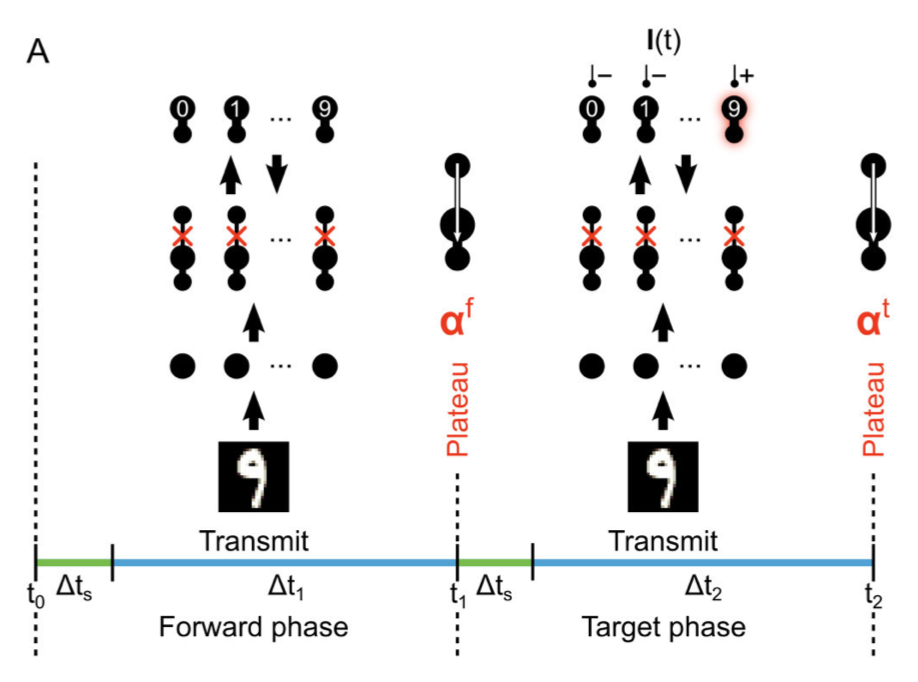
\includegraphics[scale=0.45]{../figures/report/phases}
\end{figure}

\begin{itemize}
	\item[$\to$] How is learning defined in such a model?
	Forward phase dynamics $\Leftrightarrow$ Target phase dynamics  
	
	\item[$\Rightarrow$] Somatic compartments generate Poisson process spikes:
	\begin{itemize}
		\item[$\circ$] Rates-of-fire: $\phi^l_i(t) = \phi_{max} \sigma(V_i^l(t))$
	\end{itemize}
	
	\item[$\Rightarrow$] Output Layer:
	\begin{itemize}
		\item[$\circ$] Target firing rates: $\phi_i^{1\star} = \frac{1}{\Delta t_2} \int_{t_1 + \Delta t_s}^{t_2} \phi_i^1(t)dt$
		\item[$\circ$] Loss function: $L^1 = ||\phi_i^{1\star} - \bar{\phi}_i^{1f}||_2^2 = ||\frac{1}{\Delta t_2} \int_{t_1 + \Delta t_s}^{t_2} \phi_i^1(t)dt - \frac{1}{\Delta t_1} \int_{t_0 + \Delta t_s}^{t_1} \phi_i^1(t)dt||_2^2$
	\end{itemize}
	\vspace{0.5cm}
	
	\item[$\Rightarrow$] Hidden Layer:
	\begin{itemize}
		\item[$\circ$] Target firing rates: $\phi_i^{0\star} = \bar{\phi}_i^{0f} + \alpha_i^t - \alpha_i^f$
		\item[$\circ$] Loss function: $L^0 = ||\phi_i^{0\star} - \bar{\phi}_i^{0f}||_2^2 = ||\alpha^t - \alpha^f||_2^2$
	\end{itemize}
	\vspace{0.5cm}
	
	\item[$\Rightarrow$] Local error minimization via SGD \rob{Write down gradients explicitly}
\end{itemize}




%--------------------------------------------------------------------
\newpage
\section{Empirical Investigations}

\subsection*{Scalability Across Datasets}

\begin{figure}[H]
	\centering
	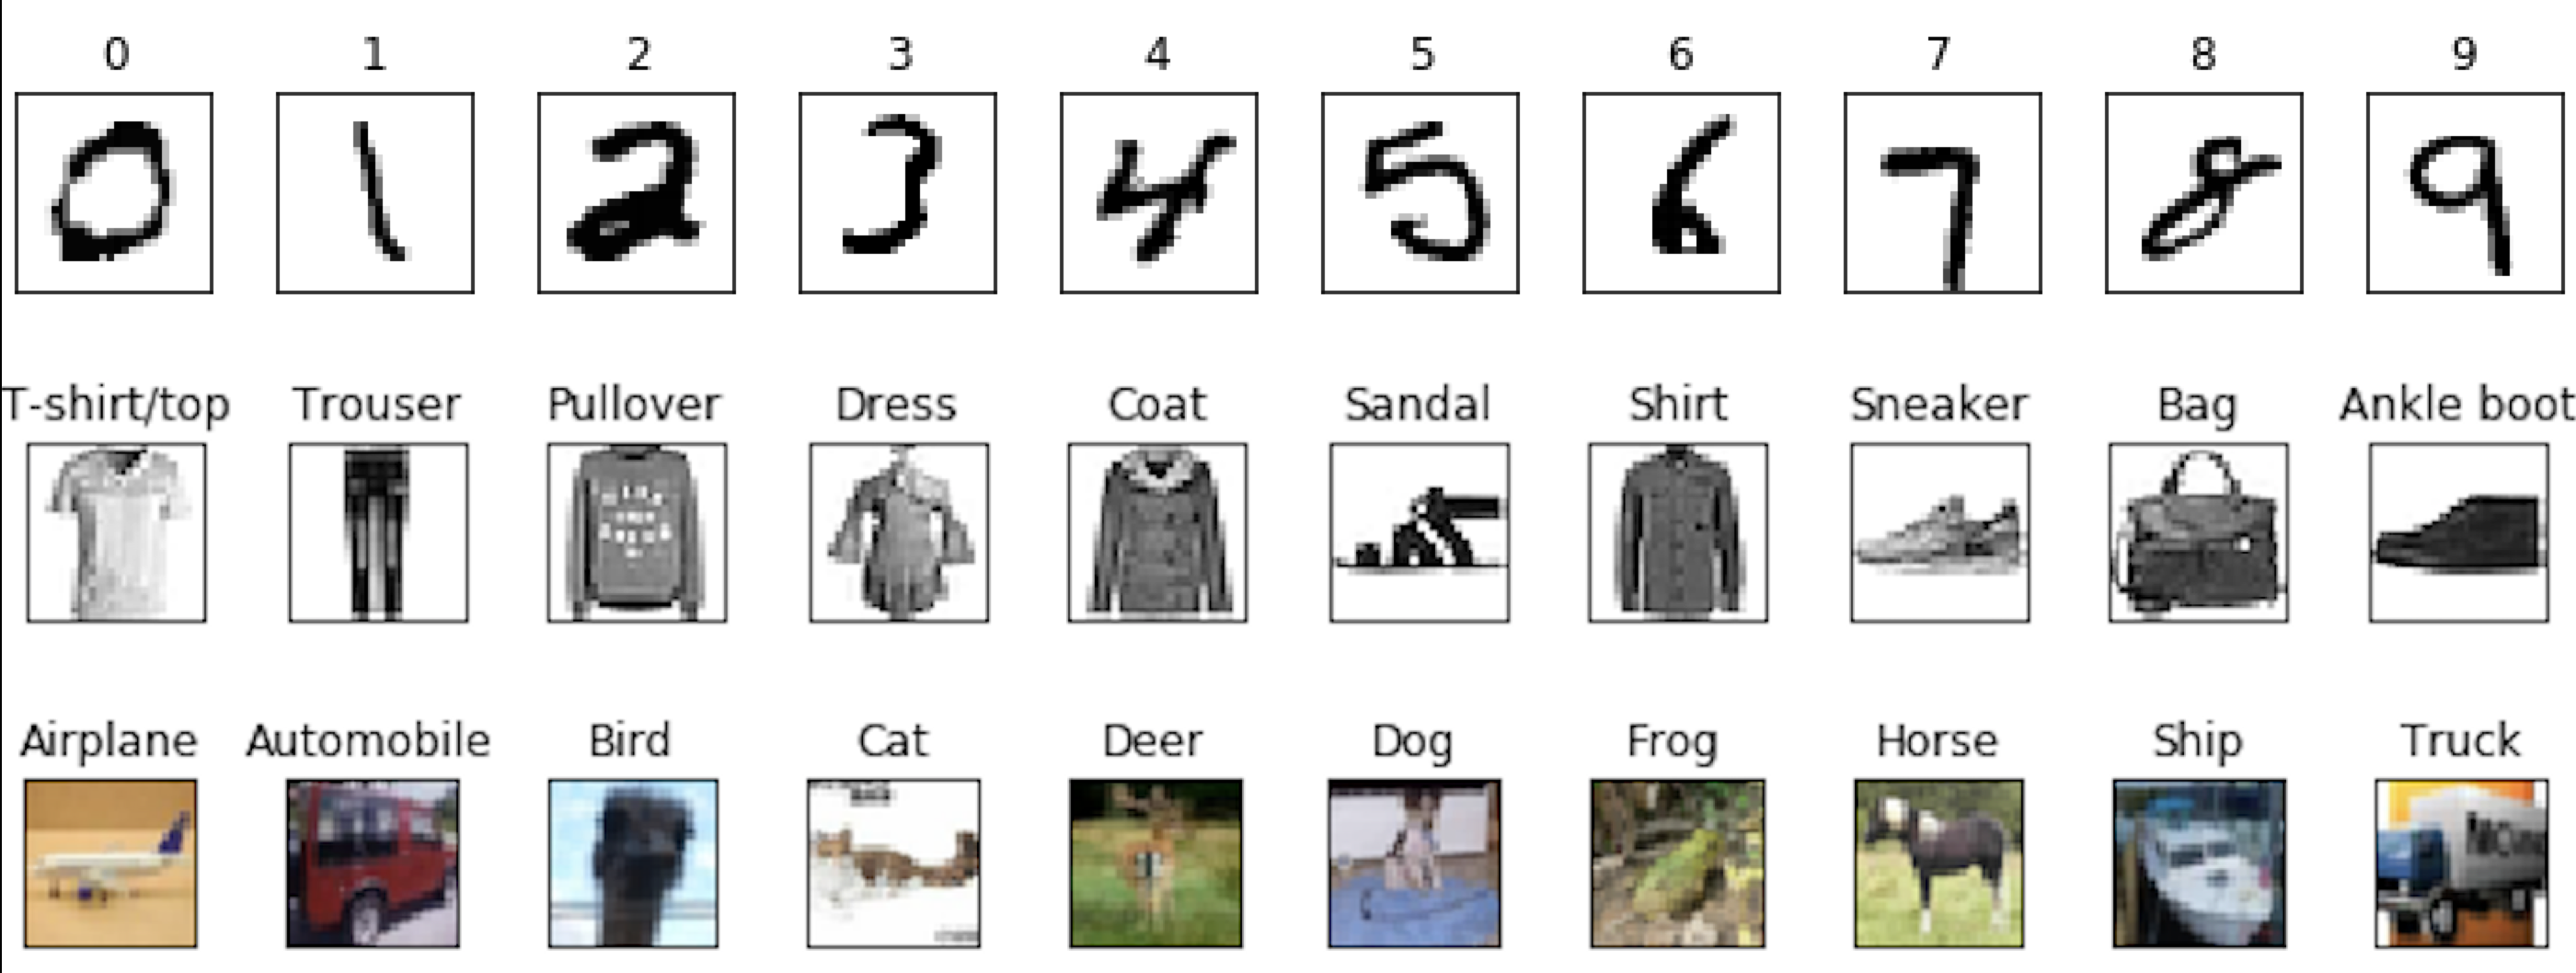
\includegraphics[width=\textwidth]{../figures/report/datasets}
	\caption{Illustration of the 10 different classes/labels of the analyzed datasets. \textbf{Top Row:} MNIST dataset. Data format: $70000 \times 1 \times 28 \times 28$. \textbf{Middle Row:} Fashion-MNIST dataset. Data format: $70000 \times 1 \times 28 \times 28$. \textbf{Bottom Row:} CIFAR-10 dataset. Data format: $60000 \times 3 \times 32 \times 32$. From top to bottom the intra-class variability/entropy increases significantly. We normalize the pixel values to lie within $[0, 1]$ and reshape the images into vector format (e.g. $X \in [0, 1]^{784}$) before training the classifiers. This helps dealing with erratic gradient behavior.}	
\end{figure}

\begin{figure}[H]
	\centering
	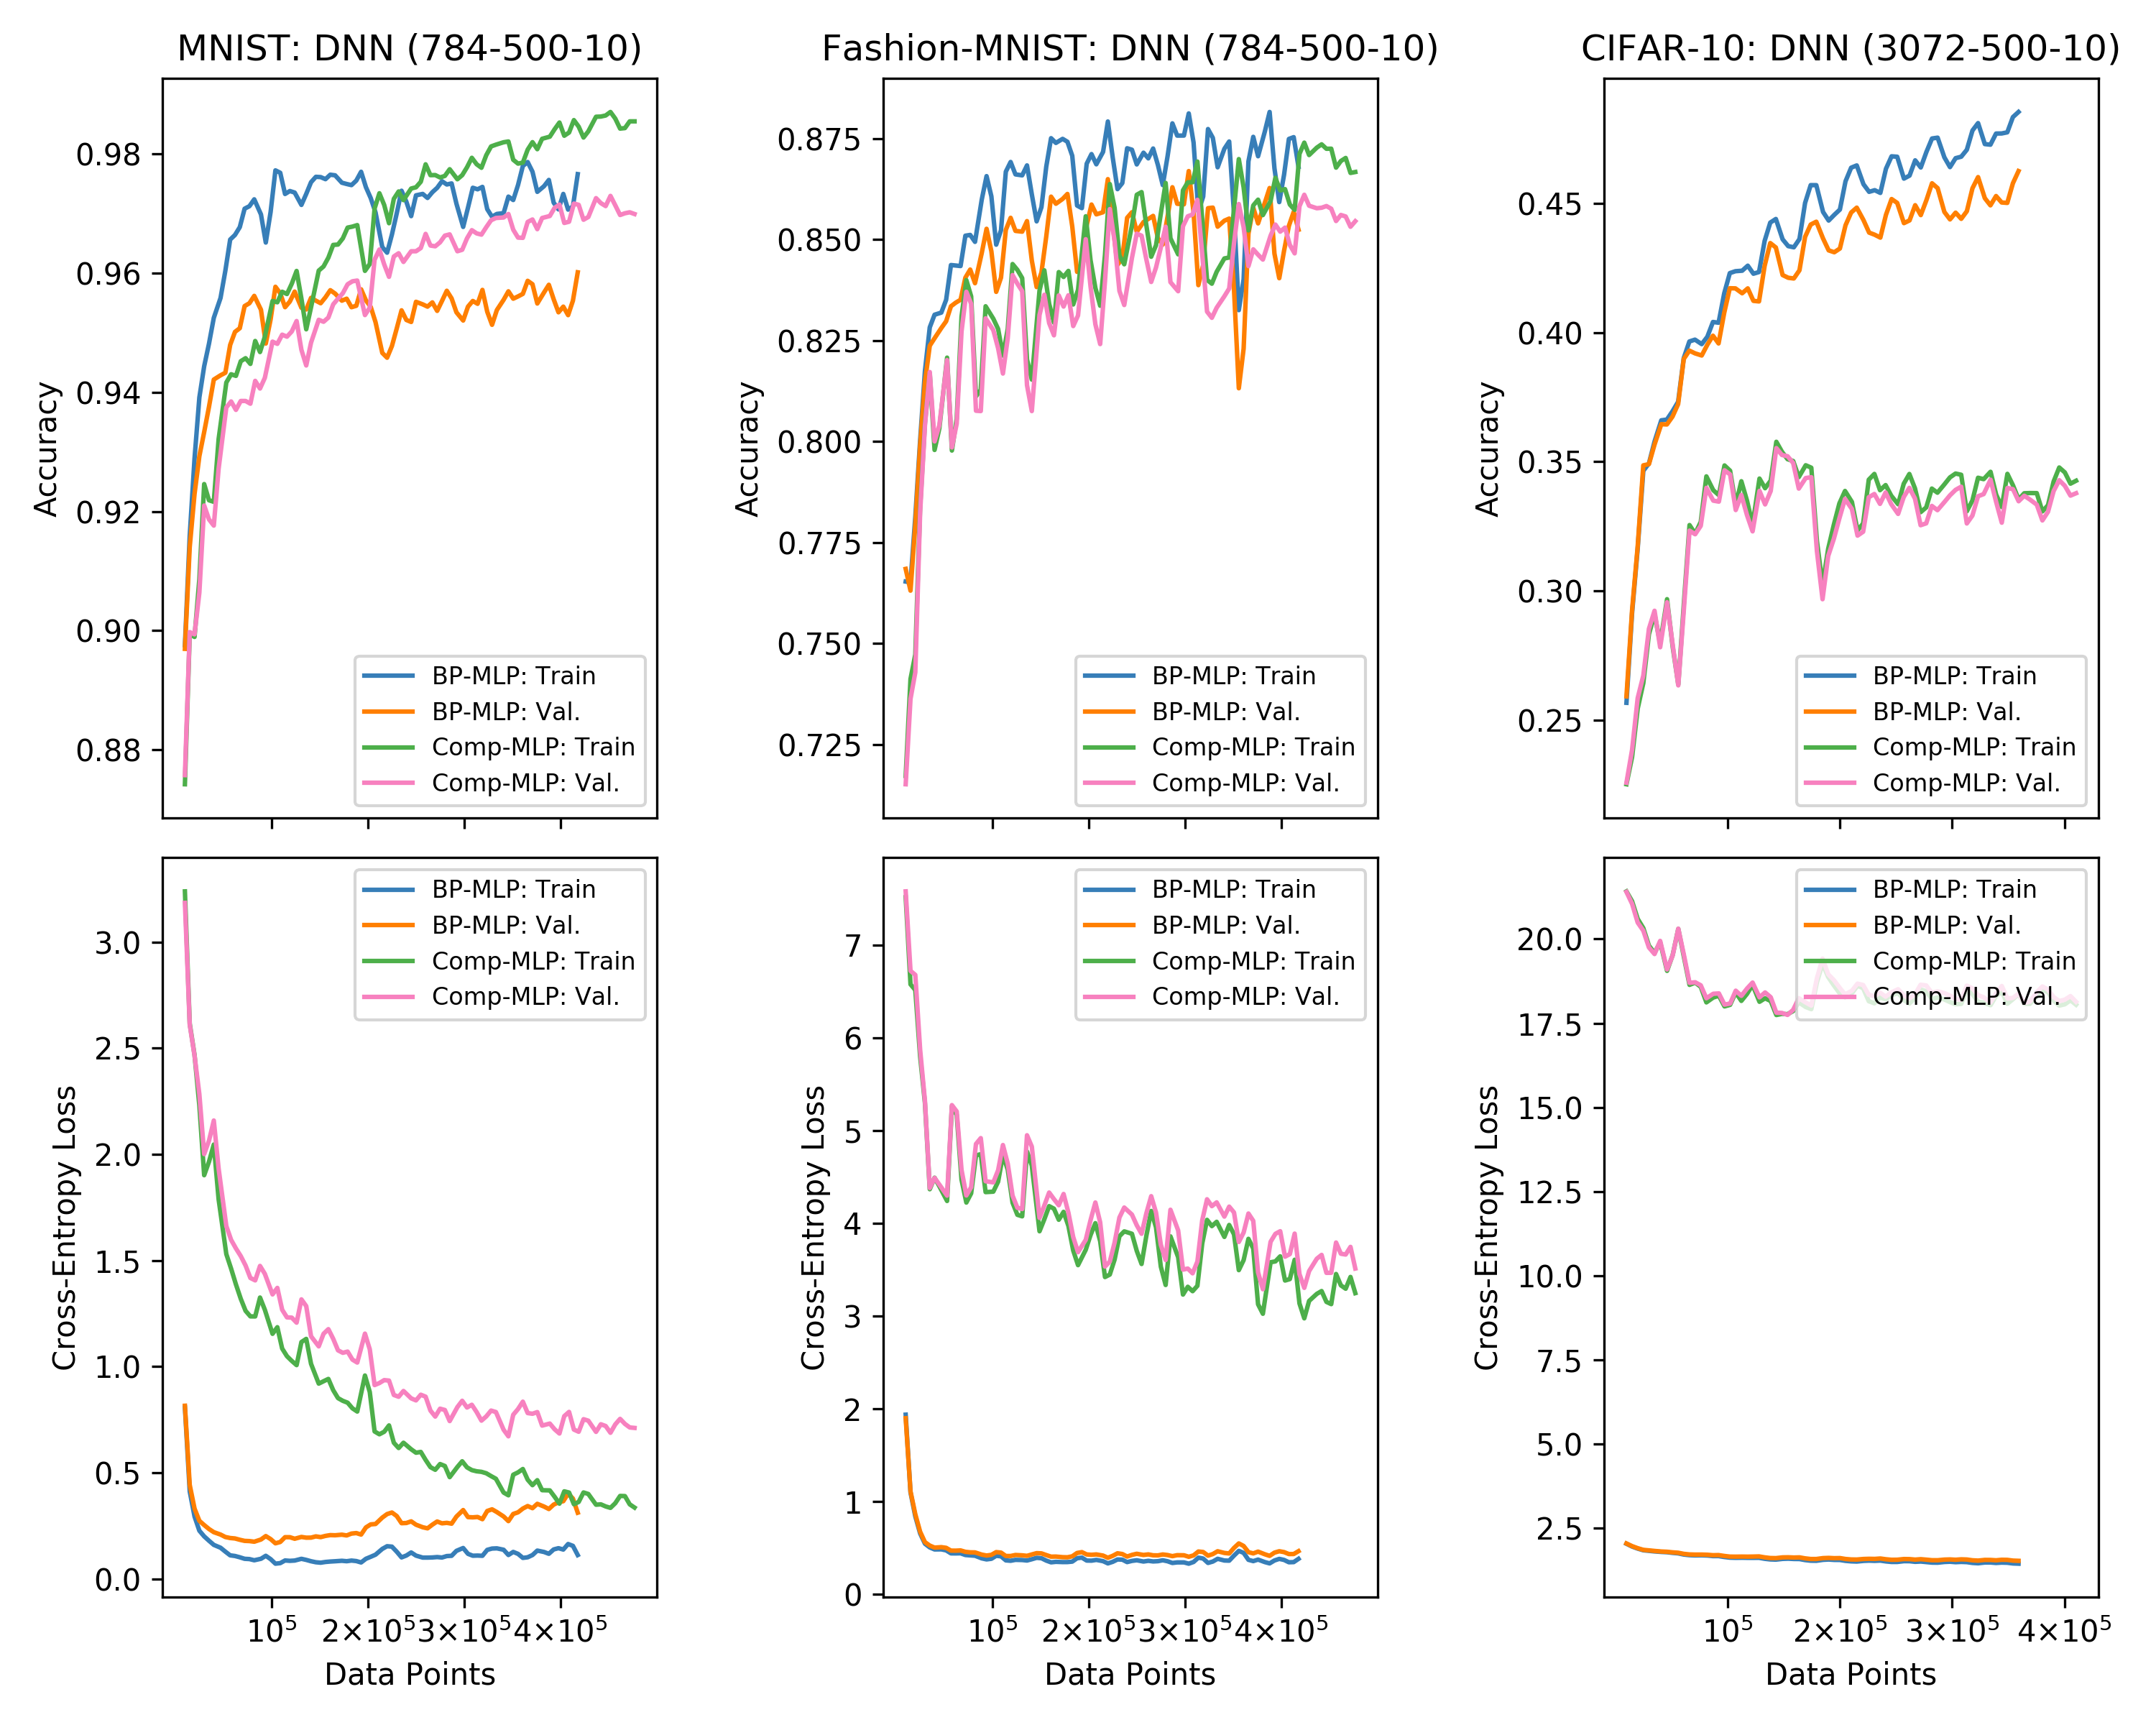
\includegraphics[width=\textwidth]{../figures/learning}
	\caption{Illustration of the learning performance.}
\end{figure}
\rob{Add description of learning performance comparison.}

\subsection*{Learning Dynamics}

\begin{figure}[H]
	\centering
	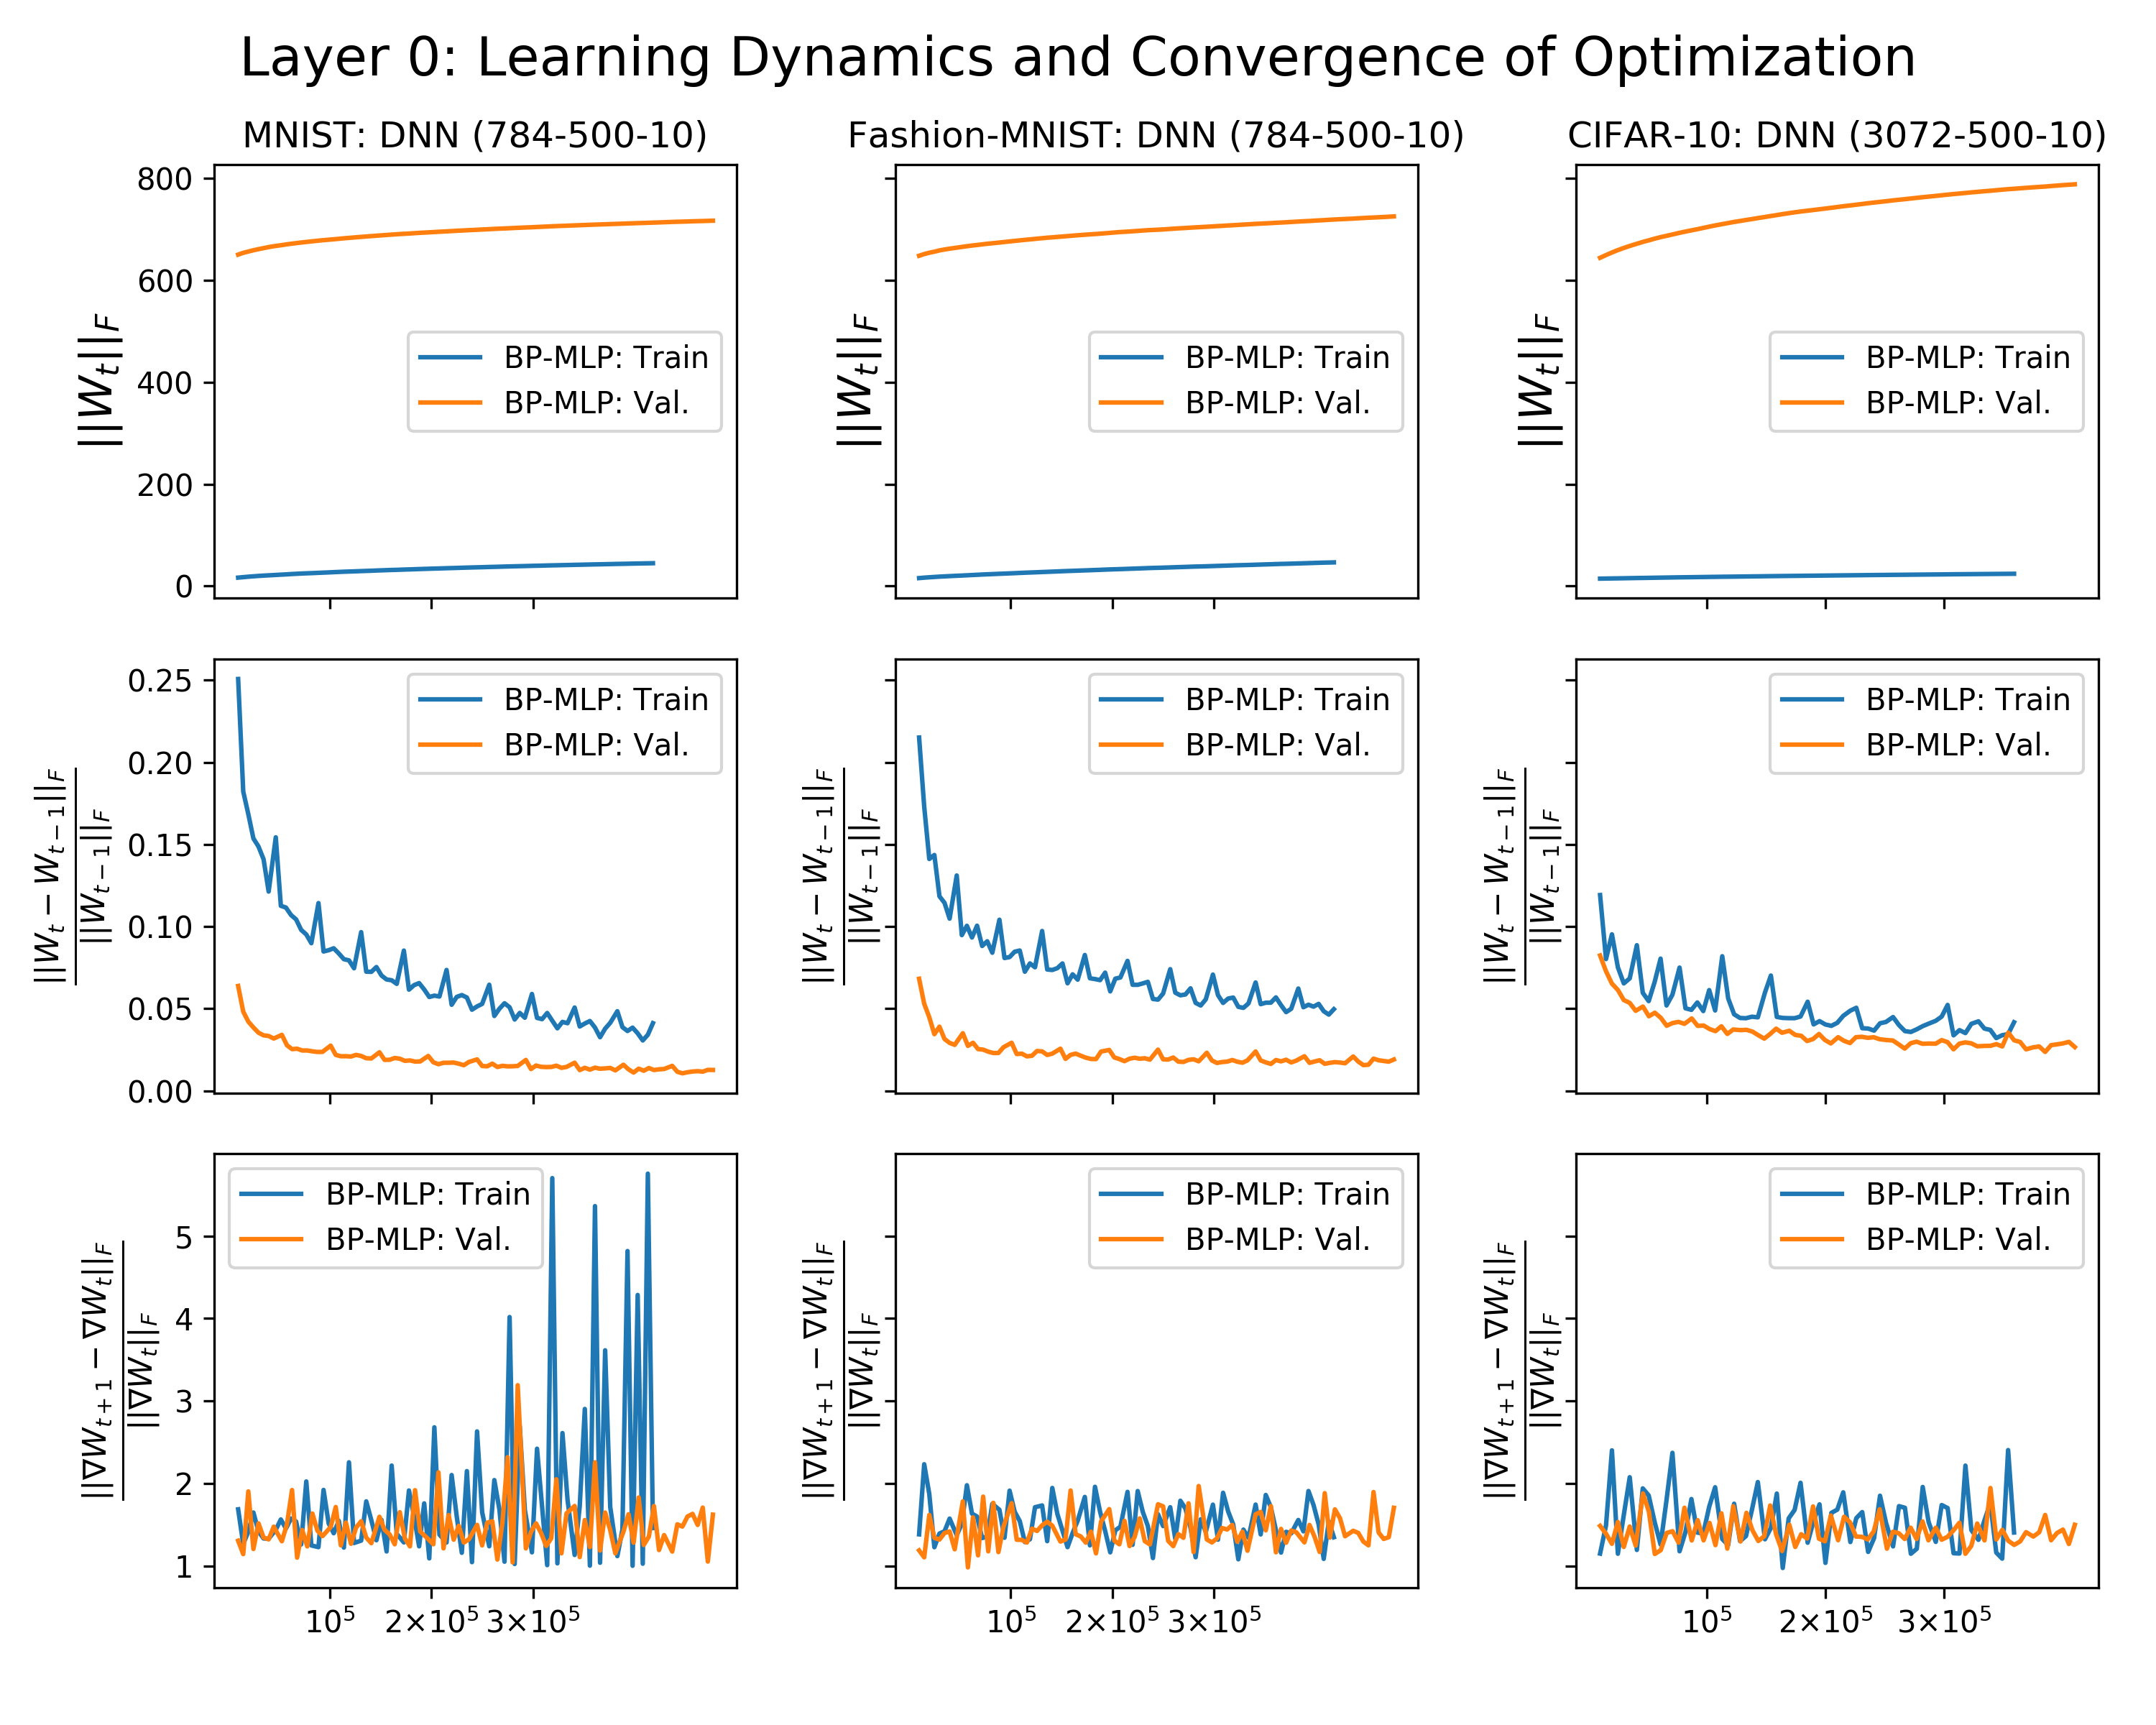
\includegraphics[width=\textwidth]{../figures/dynamics_l0}
	\caption{Illustration of the learning performance.}
\end{figure}
\rob{Add description of learning dynamics comparison.}

\newpage
\subsection*{Hyperparameter Robustness}

Bayesian Optimization \rob{Add BO classic reference} is a probabilistic technique commonly used to optimize the parameters of complex functions which are costly to evaluate. Computing cross-validated test accuracies of deep networks is one such costly function. Instead of randomly searching through the hyperparameter space, one approximates the loss function $\mathcal{L}^{k-fold}(\theta|X, y)$ with the help of a Gaussian Process (GP).

\begin{figure}[H]
	\centering
	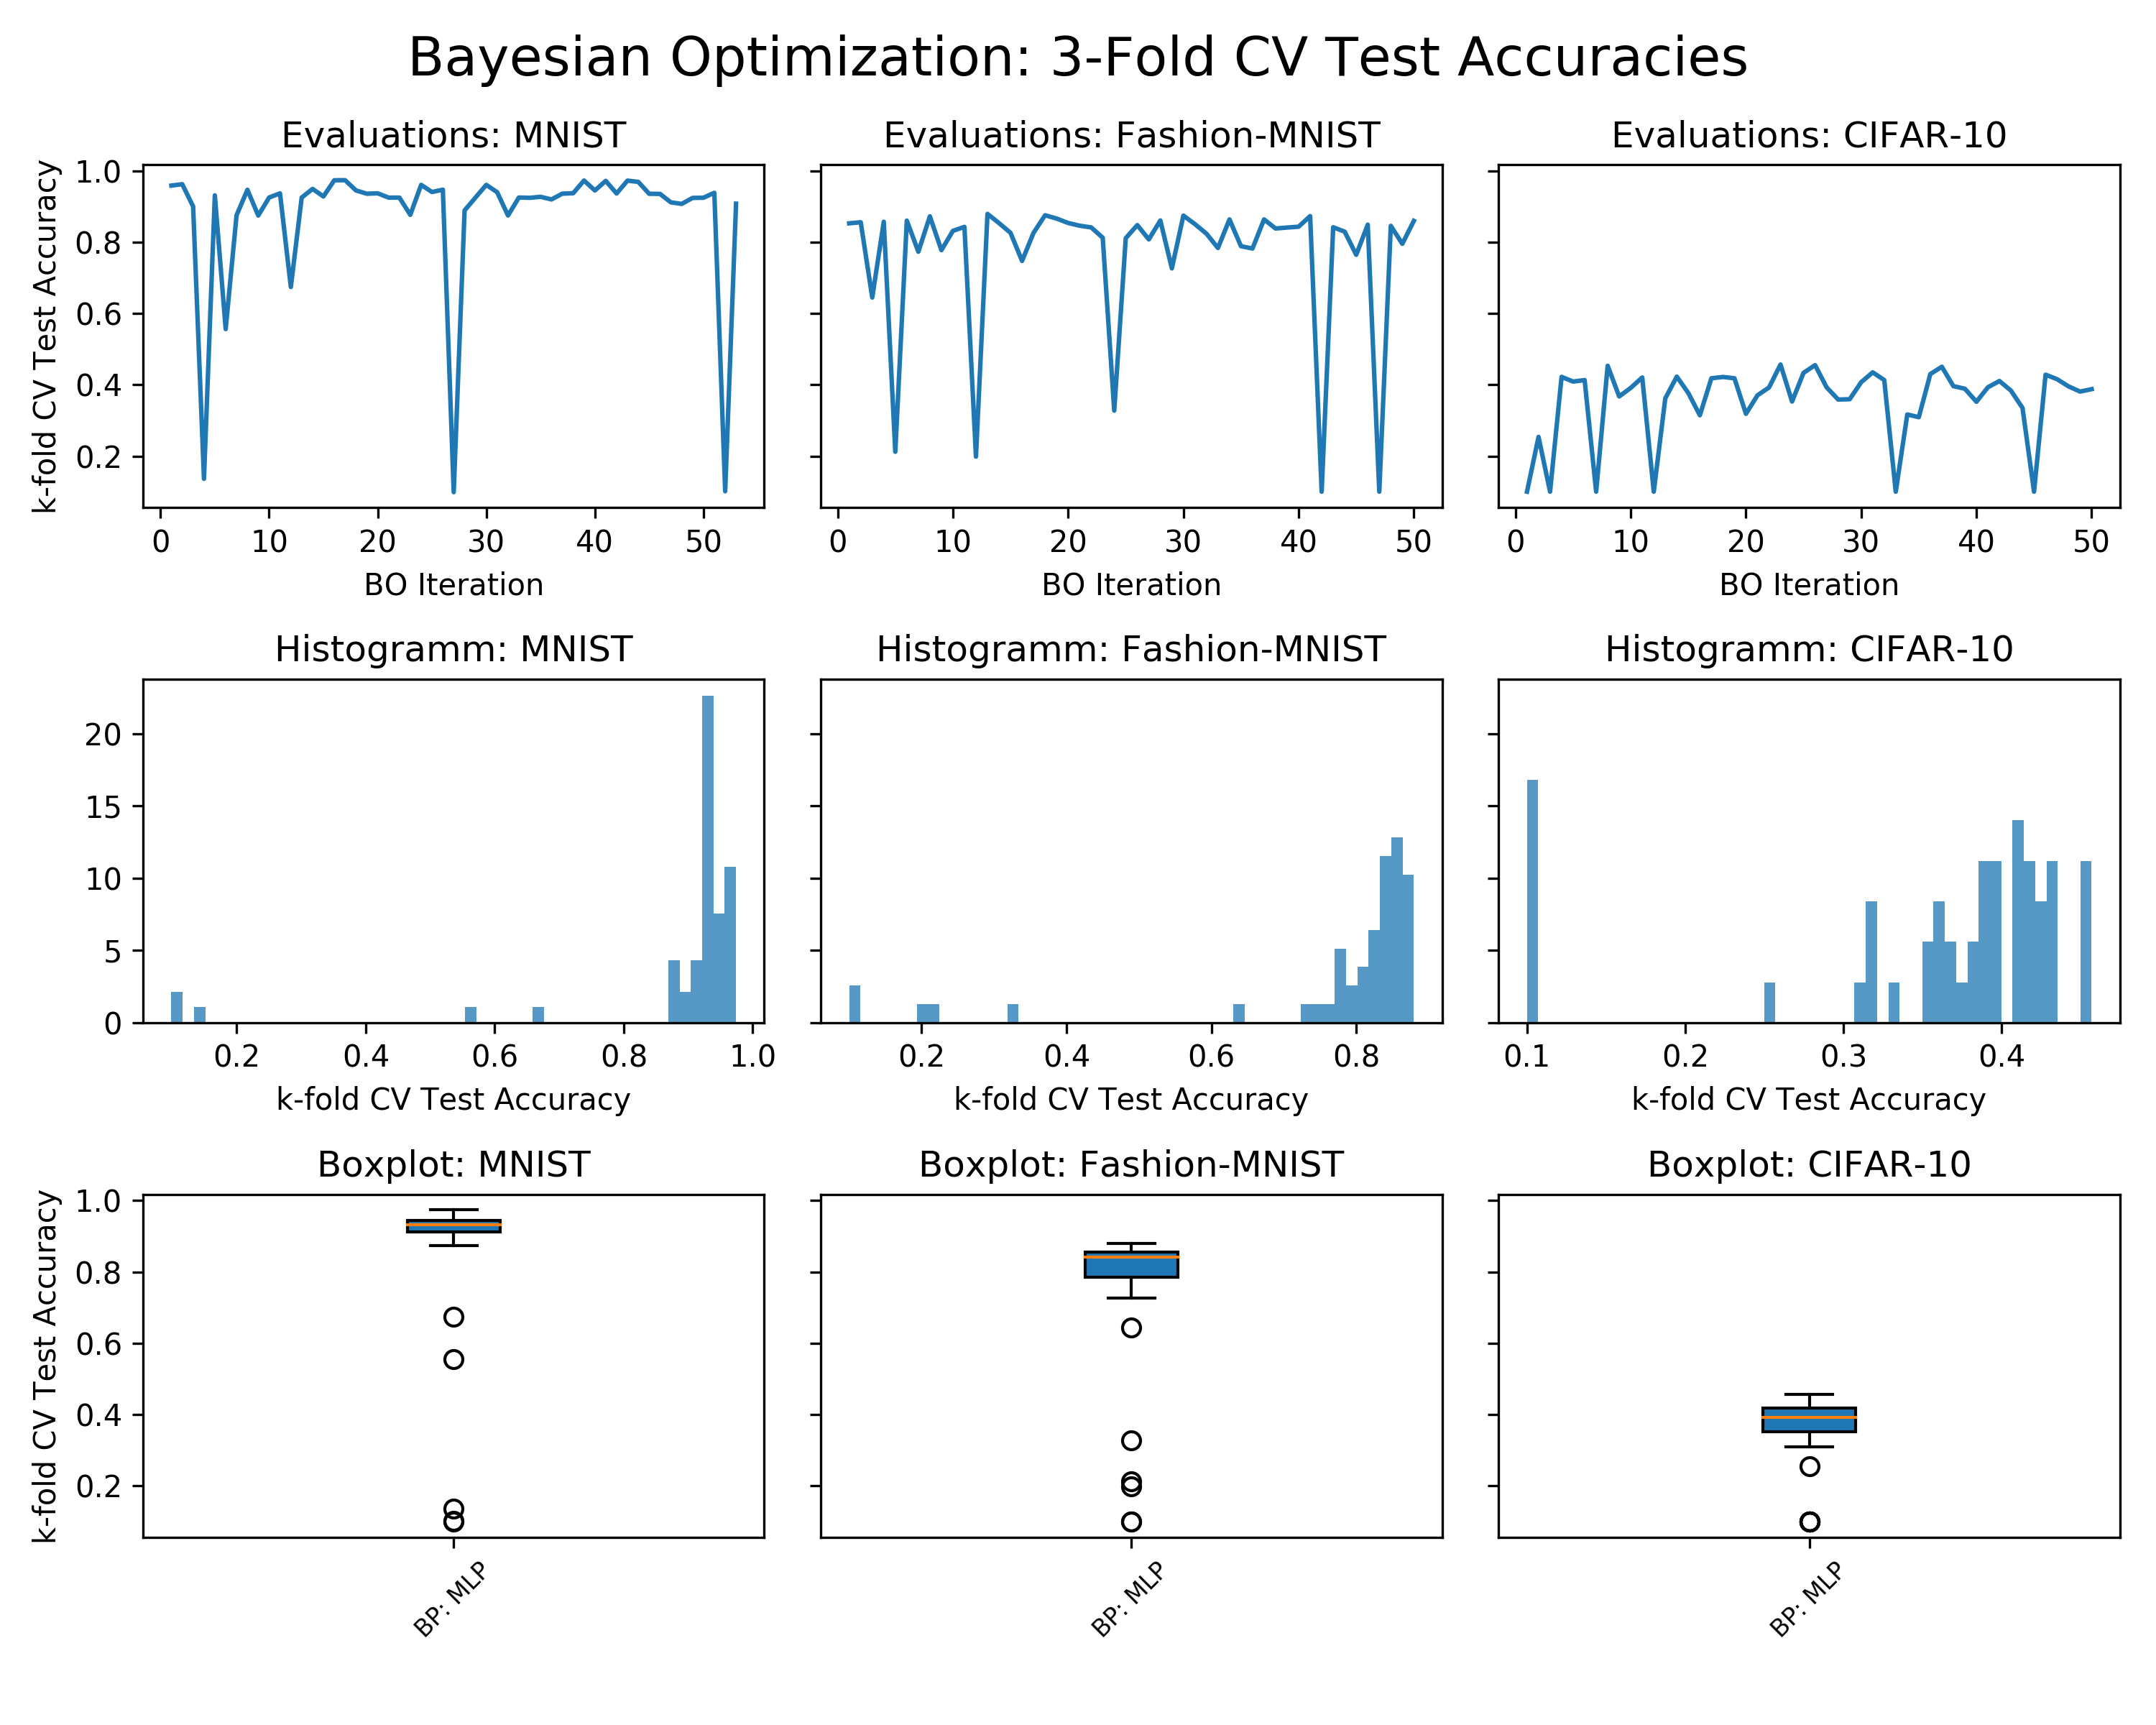
\includegraphics[width=\textwidth]{../figures/bayes_opt_comparison}
	\caption{Illustration of the learning performance.}
\end{figure}

\rob{Add description of Baysian optimization comparison.}


%--------------------------------------------------------------------
\newpage
\section{Outlook and Conclusion}

\subsection*{\citet{sacramento2018} - Dendritic Microcircuits}

General Content: MLP with simplified dendritic compartments learned in local PE plasticity fashion. No separate phases needed. Errors represent mismatch between pre input from lateral interneurons and top-down feedback. First cortical microcircuit approach. Analytically derive that such a setup/learning rule approximates backprop weight updates and proof basic performance on MNIST. Hypothesis: Pred errors are encoded at distal dendrites of pyramidal neurons - receive input from downstream neurons - in model: error arise from mismatch of lateral local interneuron inputs (SST - somatostatin) - Learning via local plasticity

Relation Guergiev: View apical dendrites as integration zones - temp difference between activity of apical dendrite in presence/absence of teaching input = error inducing plasticity at forward synapses. Used directly for learning b-u synapses without influencing somatic activity. HERE: apical dendrite has explicit error represnentation by sim integration of t-d excitation and lateral inhibition - No need for separate temporal phases - continuous operation with plasticity always turned on

* Main Results/Experiments:
    * Analytic derivation: Somatic MP at layer k integrate feedforward predictions (basal dendritic potentials) and backprop errors (apical dendritic potentials)
    * Analytic derivation: Plasticity rule converges to backprop weight change with weak feedback limit
    * Random/Fixed t-d weights = FA
    * Learned t-d weights minimizing inverse reconstruction loss = TP
    * Experiments:
        * Non-Linear regression task: Use soft rectifying nonlinearity as transfer fct - Tons of hyperparameters - injected noise current (dropout/regularization effect?)
        * MNIST - Deeper architectures: Use convex combination of learning/nudging
* Different interneuron types (PV = parvalbumin-positive) - different types of errors (generative)


In this report we have empirically investigated the robustness and learning dynamics of an alternative learning rule in deep layered structures.
We first reviewed and formalized the classical backpropagation algorithm. Afterwards, we put on computational neuroscience googles and highlighted several short-comings such as the weight transport problem as well the necessity to propagate signed errors.
In Section 3 of this report we then introduced the methodology outlined by \citet{guerguiev2017} which intends to overcome such limitations. Inspired by dendritic compartments and information integration at different sites, the algorithm solves the weight transport problem.
In Section 4 we reviewed more current approaches and compared their benefits and limitations. Thereby, we highlight the difference between behavioral and neurophysiological realism. Furthermore, we discuss the differences between learning and architecture complexity across the different approaches. 
Afterwards, we implement the approach by \citet{guerguiev2017} and compare model selection as well as hyperparameter robustness across different popular datasets. Our experiments reveal major performance decreases. This brings up the following question: Why should the brain implement a suboptimal \textbf{and} non-robust learning rule on a neurophysiological level? A simple answer to this is the flexibility that such an alternative architecture comes with.

Deep learning with ensemble multiplexing \rob{Add ideas from Blake ICLR 2018 talk}

Segregated compartments generate local targets that act as credit assignment signals in a physiologically plausible manner:
\begin{itemize}
	\item Signal can be used to exploit depth in near-continuous time
	\item \textbf{Computational} Problems
	\begin{itemize}
		\item[$\rightarrow$] Huge hyperparameter space $\to$ most likely not robust!
	\end{itemize}
	\item \textbf{Physiological} Problems
	\begin{itemize}
	\item[$\rightarrow$] How is the teaching signal internally generated?
	\item[$\rightarrow$] 2 global phases? - Length sampled from inverse Gaussian
	\item[$\rightarrow$] Stoch. gen. of plateau potentials - apical calcium spikes
	\end{itemize}
	\item[$\Rightarrow$] \citet{sacramento2018}: Neocortical micro-circuits and inhibitory interneurons might act synchronizing.
\end{itemize}
\newpage
\listoftodos[Todo-List for Rob]


%--------------------------------------------------------------------
\setlength{\bibsep}{4pt plus 0.3ex}

\bibliographystyle{ecta}%plainnat - dinat - aer - econometrics
{\footnotesize \bibliography{main.bib}}

%--------------------------------------------------------------------
\newpage
\section*{Supplementary Material}

\subsection*{A Literature Review}

\begin{figure}[H]
	\centering
	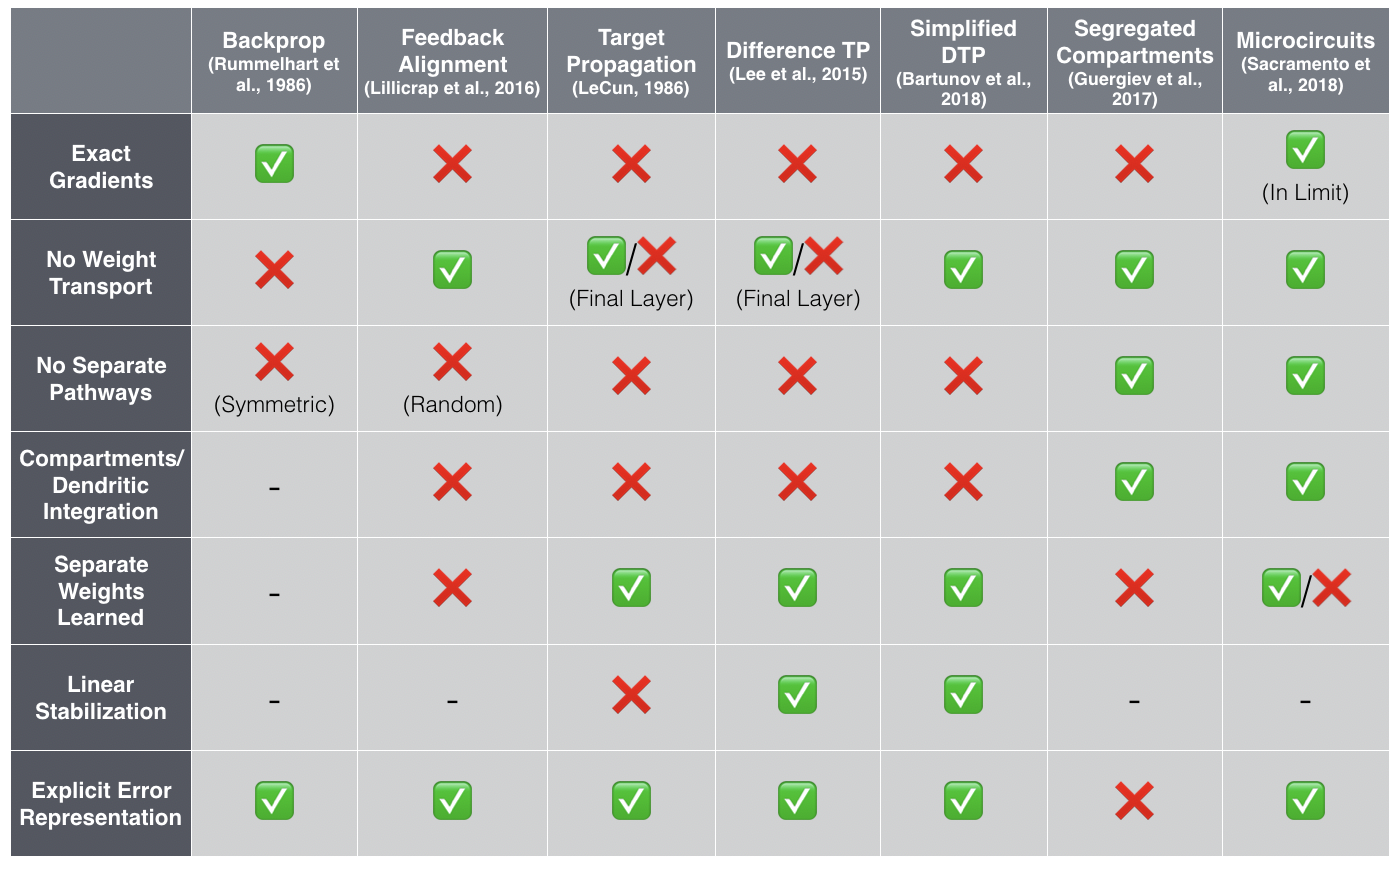
\includegraphics[width=\textwidth]{../figures/report/lit_rev}
	\caption{Literature Review.}	
\end{figure}

\subsection*{Bayesian Optimization Hyperparameter Spaces}
\rob{Add hyperparameter descriptions}

\fcolorbox{black}[HTML]{E9F0E9}{\parbox{\textwidth}{%
\small{
\begin{center}
\begin{tabular}{ |p{3cm}||p{3cm}|p{6cm}| }
 \hline
 \multicolumn{3}{|c|}{\textbf{MLP Hyperparameter Search Space:}} \\
 \hline
Hyperparameter & Range & Description\\
 \hline
 Batchsize & Integer: $[10, 500]$ & Number of data points in mini-batch\\
 Learning Rate & Float: $[0.0001, 0.05]$ & SGD learning rate\\
 \# Hidden Layers & Integer: $[1, 6]$ & \\ 
 \# Hidden Layer Units & Integer: $[30, 500]$ & \\ 
 \hline
\end{tabular}	
\end{center}
}}}

\fcolorbox{black}[HTML]{E9F0E9}{\parbox{\textwidth}{%
\small{
\begin{center}
\begin{tabular}{ |p{3cm}||p{3cm}|p{6cm}| }
 \hline
 \multicolumn{3}{|c|}{\textbf{CNN Hyperparameter Search Space:}} \\
 \hline
Hyperparameter & Range & Description\\
 \hline
 Batchsize & Integer: $[10, 500]$ & Number of data points in mini-batch\\
 Learning Rate & Float: $[0.0001, 0.05]$ & SGD learning rate\\
 \# Hidden Layers & Integer: $[1, 6]$ & \\ 
 Channels & Integer: $[3, 64]$ & \\
 Kernels & Integer: $[2, 10]$ & \\
 Stride & Integer: $[1, 3]$ & \\
 Padding & Integer: $[1, 3]$ & \\
 \hline
\end{tabular}	
\end{center}
}}}


\fcolorbox{black}[HTML]{E9F0E9}{\parbox{\textwidth}{%
\small{
\begin{center}
\begin{tabular}{ |p{3cm}||p{3cm}|p{6cm}| }
 \hline
 \multicolumn{3}{|c|}{\textbf{Compartmental DNN Hyperparameter Search Space:}} \\
 \hline
Hyperparameter & Range & Description\\
 \hline
Sparse Feedback & Boolean & Dropout 80\% of the weights\\
Conductances & Boolean & Conductances between soma and dendrites\\
Broadcast & Boolean & Feedback output to all hidden layers\\
Spiking Feedback & Boolean & \\
Spiking Feedforward & Boolean & \\
Symmetric Weights  & Boolean & Enforce symmetry\\
Noisy Symmetric W. & Boolean & Add noise to symmetric weights\\
Update Feedback W. & Boolean & Sparse feedback weights\\
Apical conductances & Boolean & Attenuated conductances apical to soma\\
Weight Optimization & Boolean & Optimize initial weights\\
Feedback Bias & Boolean & Biases in feedback weights\\
$dt$  & Float: [0, 1]& Integration time step\\
Spike Memory & Integer: $[0, 10]$ & \\
Length Forward Train & Integer: $[2, 50]$ & \\
Length Target Phase & Integer: $[2, 50]$ & \\
Length Forward Test & Integer: $[50, 100]$ &\\
$\lambda_{max}$ & Float: $[0.2, 0.5]$ & Max spike rate per time step\\
$\tau_s$ & Float: $[1, 5]$ & Synaptic time constant \\
$\tau_L$ & Float: $[7, 13]$ & Leak time constant \\
$g_B$ & Float: $[0.3, 0.9]$ & Basal conductance \\
$g_A$ & Float: $[0.02, 0.1]$ & Apical conductance \\
$E_E$ & Float: $[5, 12]$ & Excitatory Reversal Potential \\
$E_I$ & Float: $[-12, -5]$ & Inhibitory Reversal Potential \\
Forward Learning R. & Float: $[0.01, 0.05]$ & SGD learning rate for forward weights\\
Backward Learning R. & Float: $[0, 0.05]$ & SGD learning rate for backward weights\\
 \# Hidden Layers & Integer: $[1, 6]$ & \\ 
 \# Hidden Layer Units & Integer: $[30, 500]$ & \\ 
 \hline
\end{tabular}	
\end{center}
}}}

\subsection*{Notes on Reproduction}

Please clone the repository \url{https://github.com/RobertTLange/Bio-Plausible-DeepLearning} and follow the instructions outlined below:
\rob{Update readme and make ready for submission}
\hypertarget{biological-plausible-deep-learning}{%
\section{Biological Plausible Deep
Learning}\label{biological-plausible-deep-learning}}

\hypertarget{author-robert-tjarko-lange-december-2018}{%
\subsection{Author: Robert Tjarko Lange \textbar{} December
2018}\label{author-robert-tjarko-lange-december-2018}}

This project analyzes different learning rules in deep layered
structures. More specifically, we explore alternatives to
backpropagation (aka the chain rule). Weight transport (access to all
weights at every layer of the backward pass) renders backpropagation
biologically implausible. Recent alternatives explore local learning
rules and draw inspiration from the compartmental design of pyramidal
neurons.

\hypertarget{done}{%
\subsection{DONE:}\label{done}}

\begin{itemize}
\tightlist
\item
  {[}x{]} PyTorch MLP/CNN baseline for MNIST
\item
  {[}x{]} Create remote repo
\item
  {[}x{]} Generalize network architecture to variable inputs
\item
  {[}x{]} Write update\_logger, process\_logger function
\item
  {[}x{]} Plot learning curves - output from logger
\item
  {[}x{]} Add Xavier init for networks
\item
  {[}x{]} Rewrite architecture and simplify code
\item
  {[}x{]} Tried running in colab
\item
  {[}x{]} Set up bayesian optimization pipeline - BayesianOptimization

  \begin{itemize}
  \tightlist
  \item
    {[}x{]} implement cross-validation with torch data/skorch
  \item
    {[}x{]} one fct taking in hyperparams, return objective
  \item
    {[}x{]} write fct that transforms cont variables to discrete
  \item
    {[}x{]} check how to add folds/add input to eval\_nn, BO pipeline
  \item
    {[}x{]} Generalize BO pipeline to CNN
  \item
    {[}x{]} Write fct that checks if BO CNN proposal is valid
    (kernel/in/out)
  \item
    {[}x{]} Add logging to BO pipeline
  \end{itemize}
\end{itemize}

\hypertarget{todo---coding}{%
\subsection{TODO - CODING:}\label{todo---coding}}

\begin{itemize}
\tightlist
\item
  {[} {]} get\_data - Different datasets - FashionMNIST, CIFAR 10
\item
  {[} {]} Evaluate the model more frequently - not only once per epoch
\item
  {[} {]} Record weight changes
\item
  {[} {]} Get Guergiev Code running/understand
\item
  {[} {]} Restructure Guergiev code and integrate into current pipeline
\item
  {[} {]} Add comments! - Look up pep8 standard for fcts/classes
\item
  {[} {]} Work on weight visualization/changes in weights!
\item
  {[} {]} Work on error propagation comparison/delta W
  (\textbar{}\textbar{}W\_t -
  W\_t-1\textbar{}\textbar{}/\textbar{}\textbar{}W\_t\textbar{}\textbar{})
\item
  {[} {]} Runs Bayesian Opt for 10 Epochs and 50 evaluations/BO
  iterations for 3 datasets
\item
  {[} {]} Get best/worst performance, standard dev - plot as bar chart
  across approaches DNN/CNN/Guergiev
\end{itemize}

\hypertarget{todo---report}{%
\subsection{TODO - REPORT:}\label{todo---report}}

\begin{itemize}
\tightlist
\item
  {[} {]} Read papers/Add first notes of papers

  \begin{itemize}
  \tightlist
  \item
    {[}x{]} Lillicrap et al (2016)
  \item
    {[} {]} Guergiev et al (2017)
  \item
    {[}x{]} Bartunov et al (2018)
  \item
    {[}x{]} Sacramento et al (2018)
  \item
    {[} {]} Larkum (2013)
  \end{itemize}
\item
  {[} {]} Add first skeleton of report/sections - max 10 pages

  \begin{itemize}
  \tightlist
  \item
    {[} {]} Backprop/Notation
  \item
    {[} {]} Literature Notes
  \end{itemize}
\item
  {[} {]} Overview figures (Problems with backprop, Solution approaches)
\end{itemize}

\hypertarget{repository-structure}{%
\subsection{Repository Structure}\label{repository-structure}}

\begin{verbatim}
Bio-Plausible-DeepLearning
+- workspace.ipynb: Main workspace notebook - Execute for replication
\end{verbatim}

\hypertarget{how-to-use-this-code}{%
\subsection{How to use this code}\label{how-to-use-this-code}}

\begin{enumerate}
\def\labelenumi{\arabic{enumi}.}
\tightlist
\item
  Clone the repo.
\end{enumerate}

\begin{verbatim}
git clone https://github.com/RobertTLange/Bio-Plausible-DeepLearning
cd Bio-Plausible-DeepLearning
\end{verbatim}

\begin{enumerate}
\def\labelenumi{\arabic{enumi}.}
\setcounter{enumi}{1}
\tightlist
\item
  Create a virtual environment (optional but recommended).
\end{enumerate}

\begin{verbatim}
virtualenv -p python BPDL
\end{verbatim}

Activate the env (the following command works on Linux, other operating
systems might differ):

\begin{verbatim}
source BPDL/bin/activate
\end{verbatim}

\begin{enumerate}
\def\labelenumi{\arabic{enumi}.}
\setcounter{enumi}{2}
\tightlist
\item
  Install all dependencies:
\end{enumerate}

\begin{verbatim}
pip install -r requirements.txt
\end{verbatim}

\begin{enumerate}
\def\labelenumi{\arabic{enumi}.}
\setcounter{enumi}{3}
\tightlist
\item
  Run the main notebook:
\end{enumerate}

\begin{verbatim}
jupyter notebook workspace.ipynb
\end{verbatim}


\end{document}